% !TEX TS-program = xelatex
% !TEX encoding = UTF-8 Unicode

% Tennessee Technological University
% ME4140 - Fall 2016 - Fall 2017 - ? - Fall 2019 - Fall 2020 - Fall 2021
% Tristan Hill - September 10, 2020
% Turtorial 3 - Turtlesim

\documentclass[12pt]{article}
<<<<<<< HEAD
\usepackage{../../ros_tutorial}
=======
\usepackage{../../ros_tutorial} % .sty in parents parent folder
>>>>>>> 980b71026d9a2afb72b57016abcc80df0253a6a8

% Title and Misc
\newcommand{\MNUM}{3} %Module Number
\newcommand{\MNAME}{Turtlesim Testdrive} %Module Name
\pagestyle{myheadings}
\markright{{\large ME4140 - ROS Workshop - Fall 2021}}

\textwidth=7.0in
\topmargin=-0.6in
\leftmargin=0.5in
\textheight=9.25in
\hoffset=-0.5in
\footskip=0.2in

\begin{document}

\thispagestyle{plain}

\begin{center}
   {\bf \Large ROS Workshop - Tutorial\hspc\MNUM\hspc - \MNAME}\vspace{3mm}\\
   {\bf \large ME 4140 - Introduction to Robotics - Fall 2021} \vspace{5mm}\\
\end{center}

\begin{description}

\item[\textbf{\underline{Overview:}}] \hfill \vspace{3mm}\\
After completing {\it Tutorial 2 - Install ROS}, your system is setup. You are ready to begin with Turtlesim, a simplistic robot model and simulator that serves as the {\it Hello World of ROS}. You can read more about turtlesim \href{http://wiki.ros.org/turtlesim}{here} on the wiki. 

\item[\textbf{\underline{System Requirements:}}] \hfill \vspace{0mm}

\begin{itemize}
	\item {\bf ROS+OS}: This tutorial is intended for a system with ROS Melodic installed on the Ubuntu 18.04 LTS operating system. Alternate versions of ROS (i.e. - Kinetic, Noetic, etc.) may work but have not been tested. Versions of ROS are tied to versions of Ubuntu.
	\item {\bf Internet:} Your computer must be connected to the internet to proceed. Downloading and installing {\it turtlesim} will only take a few minutes.
\end{itemize}

\item[\textbf{\underline{Disclaimer:}}] \hfill \vspace{0mm}

\begin{itemize}
	\item {\bf\RD Copy and Paste Errors:} {\RD The ilearn PDF viewer does not allow the commands to be copied properly. Download the PDF if you want to copy and paste commands.} 
	
	\item {\bf Learn the Terminal:} The commands in this tutorial are relatively short, and it may help improve understanding to type them manually. {\bf Press \TABKey for auto-completion!}
	
\end{itemize}

\item[\textbf{\underline{Turtlesim Installation Instructions:}}] \hfill \vspace{0mm}

Press \CTRLKey+\ALTKey+\TKey to open a new terminal, then carefully copy each command and paste it into the terminal then press \ENTERKey. The terminal commands are shown in gray boxes, and {\bf you will have multiple terminals open at once during this tutorial.} 


\begin{enumerate}    
 
	\item Update your Ubuntu packages. It is recommended to do this before you begin something new. 

	\begin{minted}{text}
sudo apt update
	\end{minted} 
 
\item Install \href{http://wiki.ros.org/turtlesim}{turtlesim} for ROS Melodic from the pre-built repositories. This will take a few moments. Also, install a keyboard controller node.
			
\begin{minted}{text}
sudo apt install ros-melodic-turtlesim
\end{minted}

\begin{minted}{text}
sudo apt install ros-melodic-teleop-twist-keyboard
\end{minted}
	
The terminal will show if the installations were successfully, and it will indicate if the packages were previously installed (turtlesim came with ros-melodic-desktop-full).
	
\end{enumerate}	

\newpage
\item[\textbf{\underline{Turtlesim Testdrive:}}] \hfill \vspace{0mm}

Now, test the newly installed simulator. This exercise is simple, but the process is important. 

%\begin{minted}{text}
%sudo apt-get install ros-melodic-turtlesim
%\end{minted}		
%
\begin{enumerate}

\item Start the roscore in a terminal. Leave this process running and this window open. 	 

\begin{minted}{text}
roscore
\end{minted}

%\begin{minted}{text}
%roscore
%\end{minted}		

\item Open a second tab (file>new tab), and start a turtlesim\_node in the new terminal tab.

\begin{minted}{text}
rosrun turtlesim turtlesim_node
\end{minted}
%\begin{minted}{text}
%rosrun turtlesim turtlesim_node
%\end{minted}				
%
%	
%\begin{minted}{text}
% rostopic list
%\end{minted}		

			
\item In a third terminal tab run the keyboard controller node.

\begin{minted}{text}
rosrun teleop_twist_keyboard teleop_twist_keyboard.py
\end{minted}
			


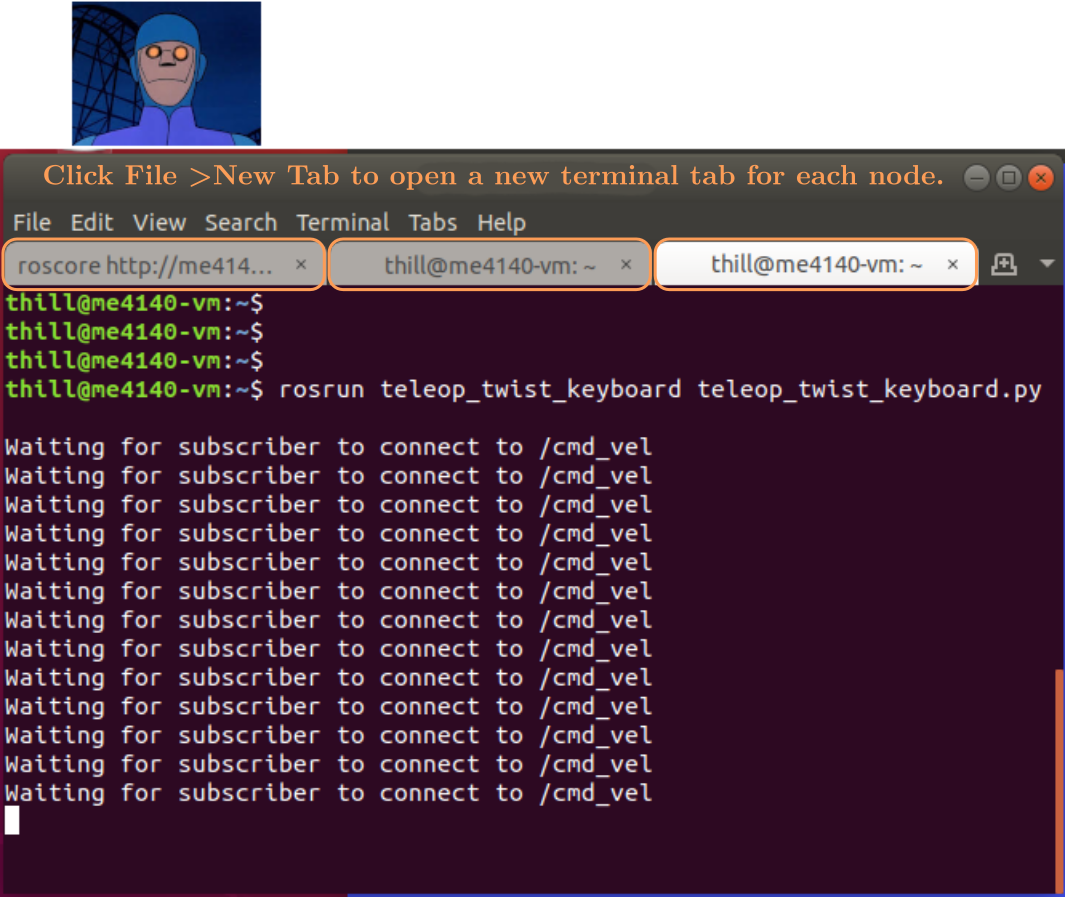
\includegraphics[scale=0.4]{tutorial3_fig3.png}	
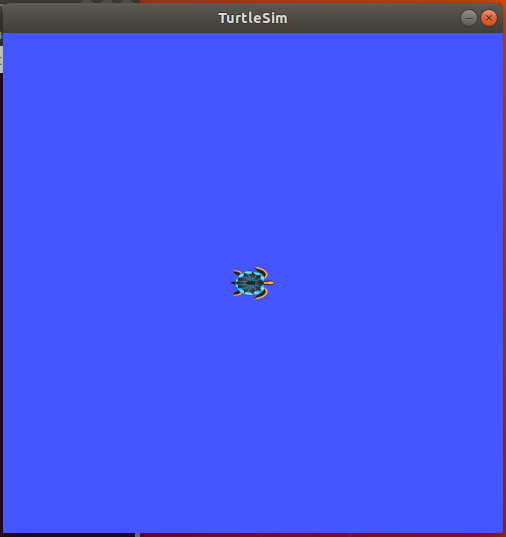
\includegraphics[scale=0.4]{tutorial3_fig2.png}	

There is a problem, the nodes are not communicating. The turtlesim node is not subscribing the to topic published by the keyboard node. \vspace{3mm}\\


\newpage
\item {\bf rostopic} is a tool in ROS for this type of problem. Try this in a new terminal with your other nodes still running.



\begin{multicols}{2}

List all available topics under master
\begin{minted}{text}
rostopic list
\end{minted}
Get info about topic: {\bf /cmd\_vel}
\begin{minted}{text}
rostopic info /cmd_vel
\end{minted}
Get info about topic: {\bf /turtle1/cmd\_vel}
\begin{minted}{text}
rostopic info /turtle1/cmd_vel
\end{minted}

\vspace{10mm} 

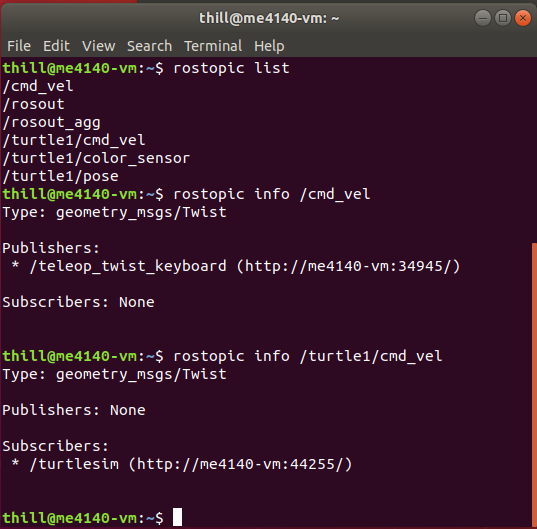
\includegraphics[scale=0.4]{tutorial3_fig4.png} \vspace{3mm}\\

\end{multicols}	
\vspace{5mm}
\item Abort the keyboard node by clicking in the third tab and pressing \CTRLKey +\CKey. Then {\bf append the following option} to the end of the keyboard node command and rerun the node. Now, the keyboard node can communicate with the turtle. 
\begin{minted}{text}
                        cmd_vel:=turtle1/cmd_vel
\end{minted}

\begin{multicols}{2}

\begin{framed}
Move the turtlesim window to the side, and select the keyboard terminal to drive using the following keys.\vspace{2mm}\\ \IKey, \JKey,\KayKey, \ELKey, and \COMMAKey (comma) \vspace{5mm}

Drive your turtle around the window and save an image of the window showing the turtle and the path. Can you drive a better ROS than shown in this picture? 
\end{framed}

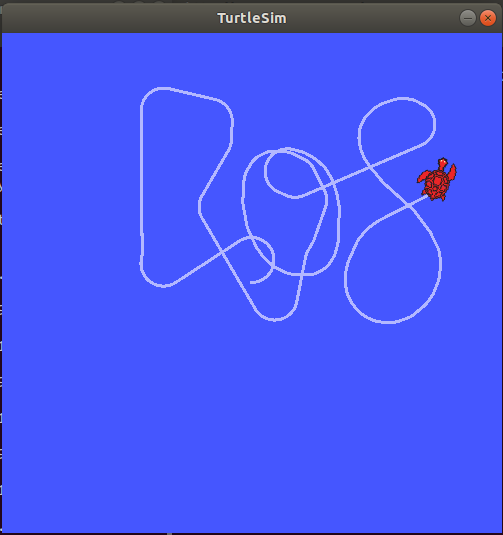
\includegraphics[scale=0.35]{tutorial3_fig1.png}	
\end{multicols}			
			
\end{enumerate}  

\item[\textbf{\underline{Tutorial Complete:}}] \hfill \vspace{3mm}\\
After completing {\it Tutorial 3 - Turtlesim}, you are ready to learn how to create a custom package to automate or the turtles behavior.

%\newpage

%\item[\textbf{\underline{Test What you have done}}]

\end{description}

\end{document}
